\documentclass{article}
\usepackage{graphicx}
\usepackage{float} %PARA QUE LAS IMÁGENES NO SEAN FLOTANTES
\floatplacement{table}{ht} 
% Paquete para ajustar los márgenes
\usepackage[margin=2.5cm]{geometry}

\usepackage{enumitem}
\usepackage{amsmath, amssymb}
% Paquete para el espaciado entre líneas
\usepackage{setspace}
\onehalfspacing

% Definición del formato del título
\title{\hrule height 5pt \\[2ex]\LARGE\bfseries Taller No.1: Cálculo de proposiciones\\[2ex] \hrule height 1.3pt \\[2ex]\LARGE }

% Redefinir el tamaño del título "Abstract"
\renewcommand{\abstractname}{\Large \textbf{Abstract}}

% Definición del formato de los autores
\usepackage{authblk}
\renewcommand\Authfont{\normalsize}
\renewcommand\Affilfont{\itshape\small}

% Puedes agregar más paquetes según tus necesidades

% Paquete para personalizar las etiquetas de sección



% Título y autores
\author{%
  \begin{minipage}[t]{0.25\textwidth}
    \centering
    \textbf{William A. Gómez Roa} \\wa.gomez@javeriana.edu.co \\ Bioingeniería y Ciencia de Datos
  \end{minipage}%
  \begin{minipage}[t]{0.25\textwidth}
    \centering
    \textbf{Luis Esteban Muñoz Sarmiento} \\ esteban@javeriana.edu.co \\ Ingeniería en Redes y Telecomunicaciones
  \end{minipage}%
}
\graphicspath{{imgs/}}
\usepackage{wasysym} 

% Eliminar la fecha
\date{}

\usepackage{changepage}

% Paquete para personalizar los títulos de sección
\usepackage{titlesec}
% Modificar el formato del título
\titleformat{\section}[hang]{\normalfont}{\thesection}{1em}{}


\begin{document}

% Título y autores sin \maketitle
\maketitle

% Ajustar los márgenes para el resumen (abstract) específicamente
% Modificar el formato del título


\begin{enumerate}
  \item Se ha definido un nuevo conectivo $\astrosun$ que tiene la siguiente tabla de verdad.

 \begin{tabular}{|c|c|c|}
  \hline
  p & q & p $\astrosun$ q \\
  \hline
  V & V & F \\
  \hline
  V & F & V \\
  \hline
   F & V & F \\
  \hline
  F & F & V \\
  \hline
\end{tabular}

Determine:
\begin{enumerate}[label=(\alph*)]
    \item Que propiedades cumple $\astrosun$:

\begin{enumerate}[label=(\alph*)]
  \item Propiedades del conectivo $\astrosun$:

  \textbf{Idempotencia}: La propiedad de idempotencia establece que aplicar el conectivo dos veces a la misma variable produce el mismo resultado. En el caso del conectivo $\astrosun$, podemos ver que no cumple con esta propiedad, ya que no siempre se obtiene el mismo resultado al aplicarlo dos veces a la misma variable. Por ejemplo, si $p$ es verdadero, entonces:

  $ p \astrosun p = F$

  Mientras que si $p$ es falso, entonces:

  $ p \astrosun p = V$

  Por lo tanto, no se cumple la propiedad de idempotencia.

  \textbf{Conmutatividad}: La propiedad de conmutatividad establece que el orden de las variables no afecta el resultado del conectivo. En el caso del conectivo $\astrosun$, no cumple con esta propiedad, ya que el resultado de $p \astrosun q$ no siempre es el mismo que el resultado de $q \astrosun p$.

  Contraejemplo:
  \begin{itemize}
    \item $V \astrosun F = V$
    \item $F \astrosun V = F$
  \end{itemize}

 

  \textbf{Asociatividad}: La propiedad de asociatividad establece que el resultado del conectivo no depende del orden en que se apliquen las operaciones. En el caso del conectivo $\astrosun$, cumple con esta propiedad, ya que el resultado es el mismo independientemente de cómo se agrupen los paréntesis.

  Ejemplo:
  \begin{itemize}
    \item $(p \astrosun q) \astrosun r = (V \astrosun V) \astrosun V = F \astrosun V = V$
    \item $p \astrosun (q \astrosun r) = V \astrosun (V \astrosun V) = V \astrosun F = V$
  \end{itemize}

  \textbf{Distributividad}: La propiedad de distributividad establece que un conectivo se puede distribuir sobre otro conectivo. En el caso del conectivo $\astrosun$, no cumple con esta propiedad, ya que no se puede distribuir sobre el conectivo $\land$ o $\lor$.

  Contraejemplo:
  \begin{itemize}
    \item $p \astrosun (q \land r) = V \astrosun (V \land V) = V \astrosun V = F$
    \item $(p \astrosun q) \land (p \astrosun r) = (V \astrosun V) \land (V \astrosun V) = V \land V = V$
  \end{itemize}

  Como podemos observar, el resultado de $p \astrosun (q \land r)$ es diferente del resultado de $(p \astrosun q) \land (p \astrosun r)$, por lo tanto, no se cumple la propiedad de distributividad.
\end{enumerate}

    
    \item Una forma equivalente a $\astrosun$ en términos de  $\land$ y $\lor$

    \begin{enumerate}
    \item Se ha definido la siguiente tabla de verdad.
    
    \begin{tabular}{|c|c|c|c|c|c|}
        \hline
        $p$ & $q$ & $p \astrosun q$ & $p \land \neg q$ & $\neg p \land q$ & $(p \land \neg q) \lor (\neg p \land q)$ \\
        \hline
        V & V & F & F & F & F \\
        V & F & V & V & F & V \\
        F & V & F & F & V & V \\
        F & F & V & F & F & F \\
        \hline
    \end{tabular}
    
    
   Por tanto, 
    
    \[ p \astrosun q \equiv (p \land \neg q) \lor (\neg p \land q) \]
    
   
    
\end{enumerate}
\end{enumerate}

  \item Demuestre que las siguientes fórmulas son equivalentes.

  \begin{enumerate}[label=\arabic*.]
    \item $(p \lor q) \rightarrow (r \land s)$
    \item $((p \lor q) \rightarrow r) \land ((p \lor q) \rightarrow s)$
  \end{enumerate}

  Demostración:

  \begin{enumerate}[label=(\alph*)]
    \item $(p \lor q) \rightarrow (r \land s)$ \quad \textbf{(Premisa inicial)}
    \item $\neg(p \lor q) \lor (r \land s)$ \quad \textbf{(Ley Alterna del Condicional)}
    \item $(\neg p \land \neg q) \lor (r \land s)$ \quad \textbf{(De Morgan)}
    \item $((\neg p \land \neg q) \lor r) \land ((\neg p \land \neg q) \lor s)$ \quad \textbf{(Ley Distributiva)}
    \item $(\neg (p \lor q) \lor r) \land (\neg (p \lor q) \lor s)$ \quad \textbf{(De Morgan)}
    \item $((p \lor q) \rightarrow r) \land ((p \lor q) \rightarrow s)$ \quad \textbf{(Ley Alterna del Condicional)}
  \end{enumerate}

  Hemos demostrado que las fórmulas 1 y 2 son equivalentes.

  \item  Determine la validez del siguiente argumento.

  Si Shakira no gana el Grammy o sus ventas disminuyen, entonces cantará solamente en inglés.
Si Shakira canta solamente en inglés, entonces descuidará el mercado hispano o se concentrará en las grabaciones. Si no se separa de Piqué, entonces no se concentrará en las grabaciones.
Ni descuida el mercado hispano ni se separa de Piqué. Por lo tanto, Shakira ganará el Grammy.

 Definiciones:
  \begin{itemize}
    \item $p$: Shakira gana el Grammy.
    \item $q$: Las ventas de Shakira disminuyen.
    \item $r$: Shakira canta solamente en inglés.
    \item $s$: Shakira descuida el mercado hispano.
    \item $t$: Shakira se concentra en las grabaciones.
    \item $u$: Shakira se separa de Piqué.
  \end{itemize}
  
  Premisas:
  \begin{enumerate}
    \item $(\neg p \lor q) \rightarrow r$ (Si Shakira no gana el Grammy o sus ventas disminuyen, entonces cantará solamente en inglés.)
    \item $r \rightarrow (s \lor t)$ (Si Shakira canta solamente en inglés, entonces descuidará el mercado hispano o se concentrará en las grabaciones.)
    \item $\neg u \rightarrow \neg t$ (Si no se separa de Piqué, entonces no se concentrará en las grabaciones.)
    \item $\neg s \land \neg u$ (Ni descuida el mercado hispano ni se separa de Piqué.)
  \end{enumerate}

\[
\begin{array}{rl}
  & (\neg p \lor q) \rightarrow r , r \rightarrow (s \lor t),
   \neg u \rightarrow \neg t,  \neg s \land \neg u
  \\
  \therefore \quad & p
\end{array}
\]
\begin{enumerate}[label=\arabic*.]
  \item \(\neg s \land \neg u\) \quad \textbf{(Premisa 4)}
  \item \(\neg u\) \quad \textbf{(Simplificación, utilizando la línea 1)}
  \item \(\neg t\) \quad \textbf{(Modus Ponendo Ponens, utilizando la premisa 3 y la línea 2)}
  \item \(\neg s\) \quad \textbf{(Simplificación, utilizando la línea 1)}
  \item \(\neg r \lor (s \lor t)\) \quad \textbf{(Alterna del Condicional de premisa 2)}
  \item \(\neg r\) \quad \textbf{(Dominación utilizando la línea 5)}
  \item \(\neg (\neg p \lor q)\) \quad \textbf{(Modus Tollendo Tollens, utilizando la premisa 1 y la línea 6)}
  \item \(p\) \quad \textbf{(Ley de De Morgan, utilizando la línea 7)}
\end{enumerate}

Hemos demostrado que el argumento es válido y que \(p\) es verdadera en esta situación específica.

Por tanto Shakira Ganarà el Grammy.

  \item  Pinocho es un niño muy mentiroso. Solo dice la verdad un día de la semana.



\begin{enumerate}
    
    \begin{itemize}
        \item Un día dijo: Yo miento los lunes y los martes.
        \item Al día siguiente dijo: Hoy es jueves, sábado o domingo.
        \item Al tercer día dijo: Yo miento los miércoles y los viernes.
    \end{itemize}
    
    \textbf{Solución:}
    
    Definamos :
    
    \begin{itemize}
        \item $p$: Pinocho dice la verdad el lunes.
        \item $q$: Pinocho dice la verdad el martes.
        \item $r$: Hoy es jueves.
        \item $s$: Hoy es sábado.
        \item $t$: Hoy es domingo.
        \item $u$: Pinocho dice la verdad el miércoles.
        \item $v$: Pinocho dice la verdad el viernes.
    \end{itemize}
    
    De acuerdo con las declaraciones de Pinocho, tenemos las siguientes premisas:
    
    \begin{enumerate}
        \item $(\neg p \land \neg q)$ \quad (Pinocho miente los lunes y los martes)
        \item $(r \lor s \lor t)$ \quad (Hoy es jueves, sábado o domingo)
        \item $(\neg u \land \neg v)$ \quad (Pinocho miente los miércoles y los viernes)
    \end{enumerate}
    
    Ahora,
    
    \begin{enumerate}
        \item Pinocho miente los lunes y los martes, por lo tanto, $\neg p$ y $\neg q$ son verdaderos.
        \item Pinocho dice la verdad el miércoles, entonces $\neg u$ es falso.
        \item Pinocho miente los miércoles y los viernes, por lo tanto, $\neg u$ y $\neg v$ son verdaderos.
    \end{enumerate}
    
    Con base en esta información, podemos llegar a las siguientes conclusiones:
    
    \begin{enumerate}
        \item Como $\neg p$ es verdadero y $\neg u$ es falso, entonces $p$ es falso (por contradicción).
        \item Como $\neg u$ y $\neg v$ son verdaderos, entonces $v$ es falso (por contradicción).
    \end{enumerate}
    
    Por lo tanto, Pinocho dice la verdad el jueves, y las demás declaraciones son falsas.
    
\end{enumerate}


  \item Utilice un CAS para construir tablas de verdad. Sugerencia: corra el archivo CDF denominado TABLAS.

En el lenguaje de programación PROLOG, se han definido las siguientes reglas y hechos que permiten llegar a las tablas de verdad. El codigo creado se muestra a continuación.
  
\begin{figure}[H]
    \centering
    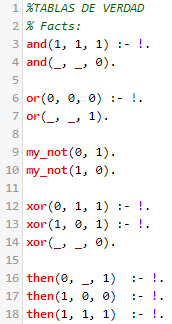
\includegraphics[width=0.3\textwidth]{code}
    \caption{Reglas y Hechos para las Tablas de Verdad}
    \label{referenciarImagenAca}
\end{figure}
Lo que se puede comprobar acá para la tabla de verdad del condicional.
\begin{figure}[H]
    \centering
    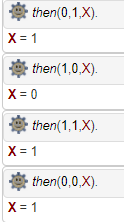
\includegraphics[width=0.2\textwidth]{prove}
    \caption{Tabla de Verdad del Condicional.}
    \label{referenciarImagenAca}
\end{figure}
  
\end{enumerate}

\end{document}
